\resizebox{\linewidth}{!}{%
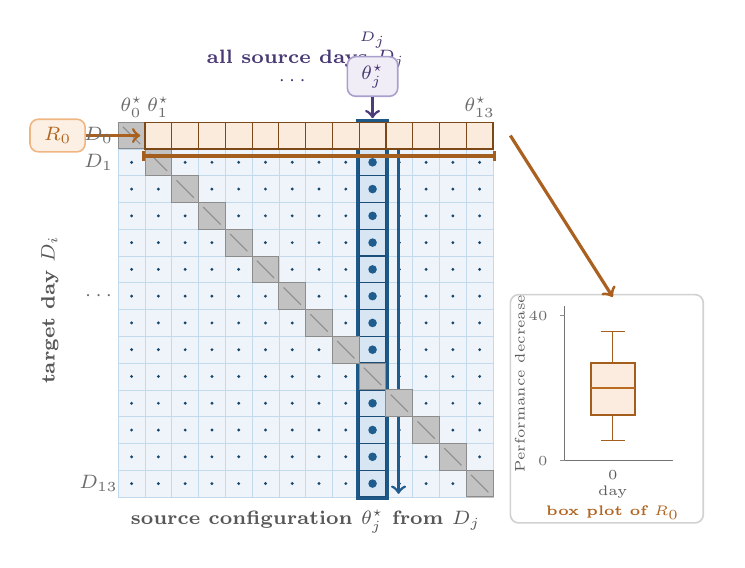
\begin{tikzpicture}[font=\sffamily\scriptsize,line width=0.58pt]
    \definecolor{dayblue}{RGB}{42,122,188}
    \definecolor{configviolet}{RGB}{103,80,164}
    \definecolor{riskorange}{RGB}{227,130,42}
    \definecolor{safegreen}{RGB}{42,150,95}

    \tikzset{
        arrow/.style={->,draw=#1!75!black,line width=1.0pt},
        every node/.style={text=black!82}
    }

    \path[use as bounding box] (0,0) rectangle (8.75,6.50);

    \def\mx{1.15}
    \def\my{5.30}
    \def\s{0.34}
    \def\targetrow{0}
    \def\sourcecol{9}

    \pgfmathsetmacro{\ytop}{\my-\targetrow*\s}
    \pgfmathsetmacro{\ycenter}{\my-\targetrow*\s-0.5*\s}
    \pgfmathsetmacro{\xsource}{\mx+\sourcecol*\s}
    \pgfmathsetmacro{\xcenter}{\mx+\sourcecol*\s+0.5*\s}

    % Base matrix.
    \foreach \r in {0,...,13}{
        \foreach \c in {0,...,13}{
            \pgfmathsetmacro{\x}{\mx+\c*\s}
            \pgfmathsetmacro{\y}{\my-\r*\s}
            \draw[draw=black!24,fill=white,line width=0.30pt] (\x,\y) rectangle ++(\s,-\s);
        }
    }

    % Step 4: repeating over all source configurations fills the off-diagonal matrix.
    \visible<4->{
        \foreach \r in {0,...,13}{
            \foreach \c in {0,...,13}{
                \ifnum\r=\c\relax
                \else
                    \pgfmathsetmacro{\x}{\mx+\c*\s}
                    \pgfmathsetmacro{\y}{\my-\r*\s}
                    \pgfmathsetmacro{\xc}{\mx+\c*\s+0.5*\s}
                    \pgfmathsetmacro{\yc}{\my-\r*\s-0.5*\s}
                    \draw[draw=dayblue!28,fill=dayblue!8,line width=0.25pt] (\x,\y) rectangle ++(\s,-\s);
                    \fill[dayblue!58!black] (\xc,\yc) circle (0.58pt);
                \fi
            }
        }
        \node[font=\bfseries\scriptsize,text=configviolet!70!black] at ({\mx+7*\s},6.10) {all source days \(D_j\)};
        \pgfmathsetmacro{\xellipsis}{\mx+6*\s+0.5*\s}
        \node[font=\scriptsize,text=configviolet!70!black] at (\xellipsis,5.82) {$\cdots$};
    }

    % Step 1: pick one source configuration column.
    \visible<1-3>{
        \foreach \r in {0,...,13}{
            \pgfmathsetmacro{\y}{\my-\r*\s}
            \draw[draw=configviolet!42,fill=configviolet!10,line width=0.34pt] (\xsource,\y) rectangle ++(\s,-\s);
        }
        \node[draw=configviolet!55,fill=configviolet!10,rounded corners=3pt,inner xsep=5pt,inner ysep=3pt,font=\bfseries\scriptsize,text=configviolet!70!black]
            (sourcecfg) at (\xcenter,5.88) {$\theta_j^{\star}$};
        \node[font=\tiny,text=configviolet!65!black] at (\xcenter,6.34) {$D_j$};
        \draw[arrow=configviolet] (sourcecfg.south) -- (\xcenter,{\my+0.05});
    }

    % Step 3: keep that configuration fixed and test it down the full target-day column.
    \visible<3>{
        \foreach \r in {0,...,13}{
            \pgfmathsetmacro{\y}{\my-\r*\s}
            \pgfmathsetmacro{\yc}{\my-\r*\s-0.5*\s}
            \draw[draw=dayblue!64!black,fill=dayblue!19,line width=0.46pt] (\xsource,\y) rectangle ++(\s,-\s);
            \fill[dayblue!76!black] (\xcenter,\yc) circle (1.55pt);
        }
        \draw[draw=dayblue!72!black,line width=1.05pt]
            ({\xsource-0.025},{\my+0.02}) rectangle ({\xsource+\s+0.025},{\my-14*\s-0.02});
        \draw[arrow=dayblue] ({\xsource+\s+0.16},{\my-0.03}) -- ({\xsource+\s+0.16},{\my-14*\s+0.04});
    }

    % Step 2: oracle diagonal excluded from transfer.
    \visible<2->{
        \foreach \d in {0,...,13}{
            \pgfmathsetmacro{\x}{\mx+\d*\s}
            \pgfmathsetmacro{\y}{\my-\d*\s}
            \draw[draw=black!45,fill=black!24,line width=0.35pt] (\x,\y) rectangle ++(\s,-\s);
            \draw[draw=black!45,line width=0.35pt] (\x+0.060,\y-0.060) -- (\x+\s-0.060,\y-\s+0.060);
        }
    }

    % Step 5: read one target row as a distribution / box plot.
    \visible<5->{
        \foreach \c in {1,...,13}{
            \pgfmathsetmacro{\x}{\mx+\c*\s}
            \draw[draw=riskorange!55!black,fill=riskorange!16,line width=0.42pt] (\x,\ytop) rectangle ++(\s,-\s);
        }
        \node[draw=riskorange!58,fill=riskorange!12,rounded corners=3pt,inner xsep=5pt,inner ysep=3pt,font=\bfseries\scriptsize,text=riskorange!78!black]
            (rowdist) at (0.38,\ycenter) {$R_0$};
        \draw[arrow=riskorange] (rowdist.east) -- ({\mx+\s-0.06},\ycenter);

        \draw[draw=riskorange!72!black,line width=1.1pt]
            ({\mx+\s-0.02},{\ytop-\s-0.09}) -- ({\mx+14*\s+0.02},{\ytop-\s-0.09});
        \draw[draw=riskorange!72!black,line width=1.1pt]
            ({\mx+\s-0.02},{\ytop-\s-0.03}) -- ({\mx+\s-0.02},{\ytop-\s-0.15});
        \draw[draw=riskorange!72!black,line width=1.1pt]
            ({\mx+14*\s+0.02},{\ytop-\s-0.03}) -- ({\mx+14*\s+0.02},{\ytop-\s-0.15});
        % Chart-style preview of the final box-plot result.
        \node[draw=black!18,fill=white,rounded corners=3pt,minimum width=2.45cm,minimum height=2.90cm,anchor=south west] at (6.12,0.20) {};
        \draw[draw=black!55,line width=0.45pt] (6.82,1.00) -- (8.20,1.00);
        \draw[draw=black!55,line width=0.45pt] (6.82,1.00) -- (6.82,2.96);
        \node[font=\tiny,text=black!64] at (7.43,0.82) {0};
        \node[font=\tiny,text=black!64] at (7.43,0.60) {day};
        \node[font=\tiny,text=black!64,rotate=90] at (6.25,1.98) {Performance decrease};
        \foreach \y/\lab in {1.00/0,2.84/40}{
            \draw[draw=black!45,line width=0.35pt] (6.76,\y) -- (6.82,\y);
            \node[font=\tiny,text=black!58,anchor=east] at (6.73,\y) {\lab};
        }
        \draw[draw=riskorange!72!black,line width=0.55pt] (7.43,1.26) -- (7.43,2.64);
        \draw[draw=riskorange!72!black,line width=0.55pt] (7.28,1.26) -- (7.58,1.26);
        \draw[draw=riskorange!72!black,line width=0.55pt] (7.28,2.64) -- (7.58,2.64);
        \draw[draw=riskorange!72!black,fill=riskorange!15,line width=0.65pt] (7.15,1.58) rectangle (7.71,2.24);
        \draw[draw=riskorange!82!black,line width=0.75pt] (7.15,1.92) -- (7.71,1.92);
        \node[font=\bfseries\tiny,text=riskorange!78!black] at (7.43,0.34) {box plot of $R_0$};
        \draw[arrow=riskorange,line width=1.15pt] ({\mx+14*\s+0.22},\ycenter) -- (7.43,3.08);
    }

    % Sparse numeric anchors after overlays so they remain readable.
    \foreach \c/\lab in {0/$\theta_0^{\star}$,1/$\theta_1^{\star}$,13/$\theta_{13}^{\star}$}{
        \pgfmathsetmacro{\x}{\mx+\c*\s+0.5*\s}
        \node[font=\scriptsize,text=black!58] at (\x,5.49) {\lab};
    }
    \foreach \r/\lab in {0/$D_0$,1/$D_1$,6/$\cdots$,13/$D_{13}$}{
        \pgfmathsetmacro{\y}{\my-\r*\s-0.5*\s}
        \node[font=\scriptsize,text=black!58] at (0.90,\y) {\lab};
    }

    \node[font=\bfseries\scriptsize,text=black!66]
        at ({\mx+7*\s},0.23) {source configuration $\theta_j^{\star}$ from $D_j$};
    \node[font=\bfseries\scriptsize,text=black!66,rotate=90]
        at (0.28,{\my-7*\s}) {target day $D_i$};
\end{tikzpicture}%
}
